% chapter05.tex

 %%%%%%%%%%%%%%%%%%%%%%%%%%%%%%%%%%%%%%%%%%%%%%%%%%%%%%%%%%%%%%%%%%%%%%%%%%%%%
 %                                                                           %
 %    PyMS documentation                                                     %
 %    Copyright (C) 2005-8 Vladimir Likic                                    %
 %                                                                           %
 %    The files in this directory provided under the Creative Commons        %
 %    Attribution-NonCommercial-NoDerivs 2.1 Australia license               %
 %    http://creativecommons.org/licenses/by-nc-nd/2.1/au/                   %
 %    See the file license.txt                                               %
 %                                                                           %
 %%%%%%%%%%%%%%%%%%%%%%%%%%%%%%%%%%%%%%%%%%%%%%%%%%%%%%%%%%%%%%%%%%%%%%%%%%%%%

\chapter{Data pre-processing}

\section{Noise smoothing}

The purpose of noise smoothing is to remove high-frequency noise from
data, and thereby increase the contribution of the signal relative to
the contribution of the noise.

\subsection{Window averaging}

\noindent
[ {\em This example is in pyms-test/50} ]

A simple approach to noise smoothing is moving average window smoothing.
In this approach the window of a fixed size ($2N+1$ points) is moved
across the ion chromatogram, and the intensity value at each point is
replaced with the mean intensity calculated over the window size.
The example below illustrates smoothing of TIC by window averaging.

Load the data and get the TIC:

\begin{verbatim}
>>> andi_file = "/x/PyMS/data/gc01_0812_066.cdf"
>>> data = ANDI_reader(andi_file)
 -> Reading netCDF file '/x/PyMS/data/gc01_0812_066.cdf'
>>> tic = data.get_tic()
\end{verbatim}

Apply the mean window smooting with the 5-point window:

\begin{verbatim}
from pyms.Noise.SavitzkyGolay import window_smooth
tic1 = window_smooth(tic, window=5)
 -> Window smoothing (mean): the wing is 2 point(s)
\end{verbatim}

Apply the median window smooting with the 5-point window:

\begin{verbatim}
>>> tic2 = window_smooth(tic, window=5, median=True)
 -> Window smoothing (median): the wing is 2 point(s)
\end{verbatim}

Apply the mean windows smoothing, but specify the window as
a time string (in this example, 7 seconds):

\begin{verbatim}
>>> tic3 = window_smooth(tic, window='7s')
 -> Window smoothing (mean): the wing is 9 point(s)
\end{verbatim}

Time strings are explained in the Section \ref{sec:time-string}.
The effects of the moving window average smoothing are shown in
Figures \ref{fig:smoothed-mean} and \ref{fig:smoothed-median}.

\begin{figure}[htp]
\begin{center}
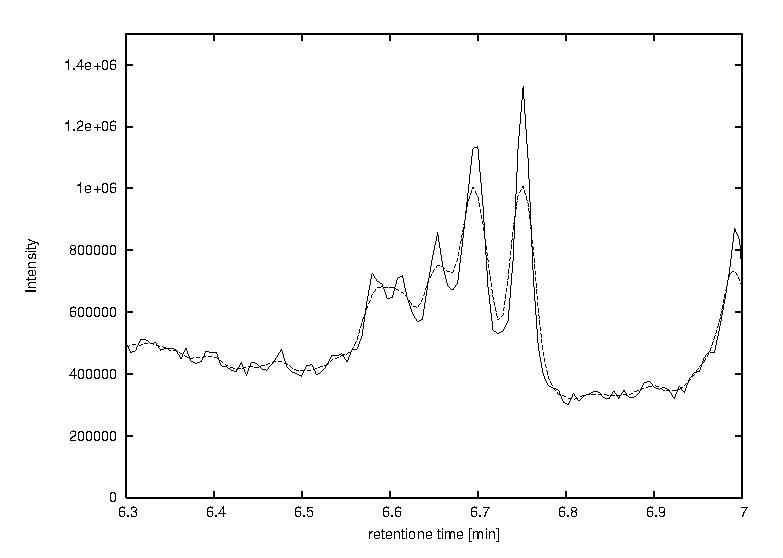
\includegraphics{graphics/50/tic_mean_smoothed.eps}
\caption{The effect of the 5-point mean moving window average smoothing
on the TIC from 'gc01\_0812\_066' data set. The segment 7.0--8.0
minutes is shown. The original TIC is shown in full line, the smoothed
TIC is shown in dashed line.}
\label{fig:smoothed-mean}
\end{center}
\end{figure}

\begin{figure}[htp]
\begin{center}
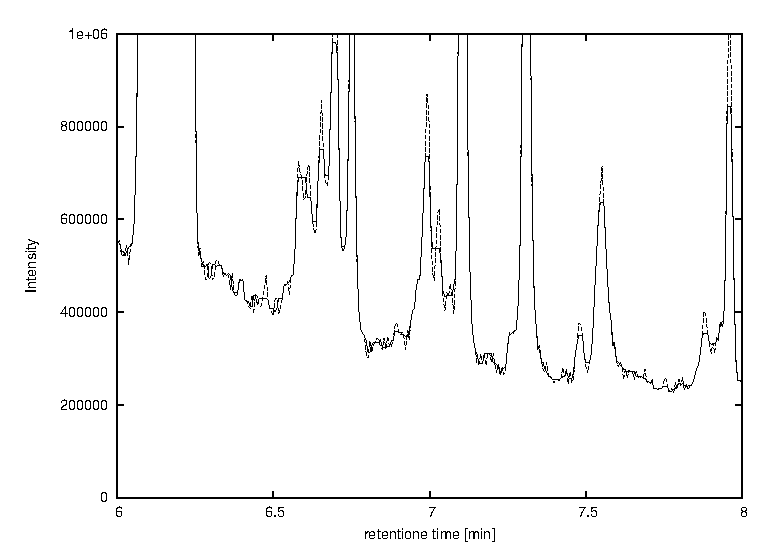
\includegraphics{graphics/50/tic_median_smoothed.eps}
\caption{The effect of the 5-point median moving window average smoothing
on the TIC from 'gc01\_0812\_066' data set. The segment 7.0--8.0
minutes is shown. The original TIC is shown in full line, the smoothed
TIC is shown in dashed line.}
\label{fig:smoothed-median}
\end{center}
\end{figure}

\subsection{Savitzky--Golay noise filter}

\noindent
[ {\em This example is in pyms-test/51} ]

A more sophisticated noise filter is the Savitzky-Golay filter.
Given the data loaded as above, this filter can be applied as
follows:

\begin{verbatim}
>>> from pyms.Noise.SavitzkyGolay import savitzky_golay
>>> tic1 = savitzky_golay(tic)
 -> Applying Savitzky-Golay filter
      Window width (points): 7
      Polynomial degree: 2
\end{verbatim}

In this example the default parameters were used.

\section{Time strings}
\label{sec:time-string}

A time string is specification of time interval, that takes the format
'NUMBERs' or 'NUMBERm' for time interval in seconds or minutes. For
example, these are valid time strings: '10s' (10 seconds) and '0.2m'
(0.2 minutes).


